\begin{frame}
\frametitle{Plane wave solutions of the Dirac equation}
For a particle at rest, $\va{p} = 0$ and the Dirac equation becomes:
\[
i\gamma^0\partial_0\psi = m \psi, \,\,\, or \, \, \,  i \mqty(1 & 0 & 0 & 0\\ 0 & 1 & 0 & 0 \\
0 & 0 & -1 & 0 \\ 0 & 0 & 0 & -1 ) \ \mqty(\dot{\psi_1} \\ \dot{\psi_2}\\ \dot{\psi_3} \\ \dot{\psi_4}) = 
m \mqty(\psi_1 \\ \psi_2\\ \psi_3 \\ \psi_4)
\]
There are four independent solutions. How do we interpret these?
\[
\psi^{(1)} = w^{(1)} e^{-i m\cdot t}, \,\,\, \psi^{(2)} = w^{(2)} e^{-i m\cdot t}, \,\,\,
\psi^{(3)} = w^{(3)} e^{+i m\cdot t}, \,\,\, \psi^{(4)} = w^{(4)} e^{i m\cdot t}
\]
\[
w^{(1)} = \mqty(1 \\ 0 \\ 0 \\ 0), \,\,\, w^{(1)} = \mqty(0\\ 1 \\ 0 \\ 0), \,\,\,
w^{(3)} = \mqty(0 \\ 0 \\ 1 \\ 0), \,\,\, w^{(4)} = \mqty(0 \\ 0 \\ 0 \\ 1), \,\,\,
\]

\end{frame}
\begin{frame}
\frametitle{The solutions are eigenvalues of the spin}
The solutions are eigenvalues of the z-component of the spin, $\Sigma_3$, which in the Dirac representation is:
\[
\Sigma_3 = \mqty(\sigma_3 & 0 \\ 0 &  \sigma_3) = \mqty(1 & 0 & 0 & 0\\ 0 & -1 & 0 & 0 \\
0 & 0 & 1 & 0 \\ 0 & 0 & 0 & -1 )
\]
thus:
\[
\psi^{(1)} : \Sigma_3 = +1, \,\,\,
\psi^{(2)} : \Sigma_3 = -1, \,\,\,
\psi^{(3)} : \Sigma_3 = +1, \,\,\,
\psi^{(4)} : \Sigma_3 = -1.
\]

Thus, we can see that two solutions of the Dirac equation corresponde to spin-up and spin-down. 
\end{frame}
%
\begin{frame}
\frametitle{Negative energy solutions}

Since we define the eigenvalue of the operator $\pdv{t}$~to be the energy, we find that 
$\psi^{(1)}$~and $\psi^{(2)}$~are positive energy solutions and 
$\psi^{(3)}$~and $\psi^{(4)}$~are negative energy solutions.

\begin{alertblock}{Surprise!}
Dirac's equation \alert{predicts} negative energy solutions.
\end{alertblock}
\end{frame}
%
\begin{frame}
\frametitle{Dirac struggle with negative energy solutions: protons}

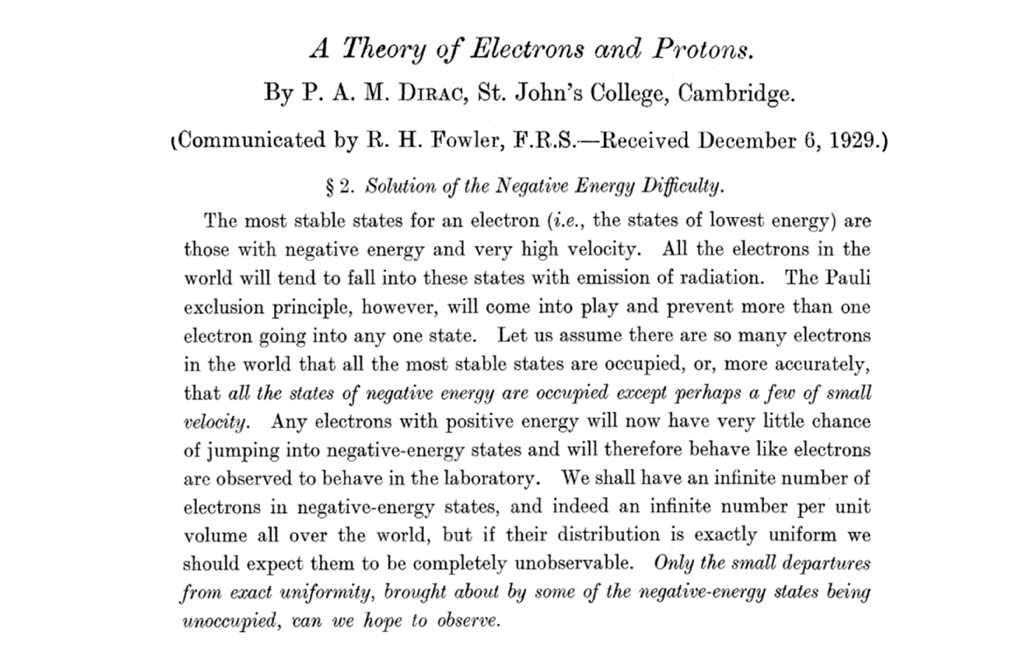
\includegraphics[scale=0.3]{img/DiracElectronProton.png}
\end{frame}

\begin{frame}
\frametitle{The opinion of Heisemberg}

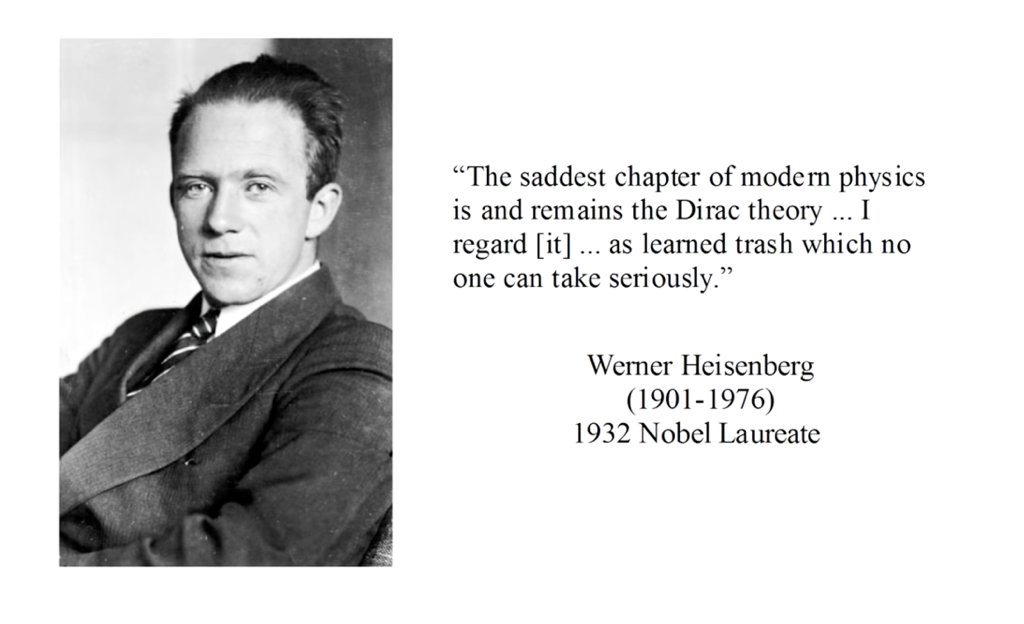
\includegraphics[scale=0.3]{img/HeisembergOpinionDirac.png}
\end{frame}

\begin{frame}
\frametitle{Identifying holes in the negative sea with positrons}

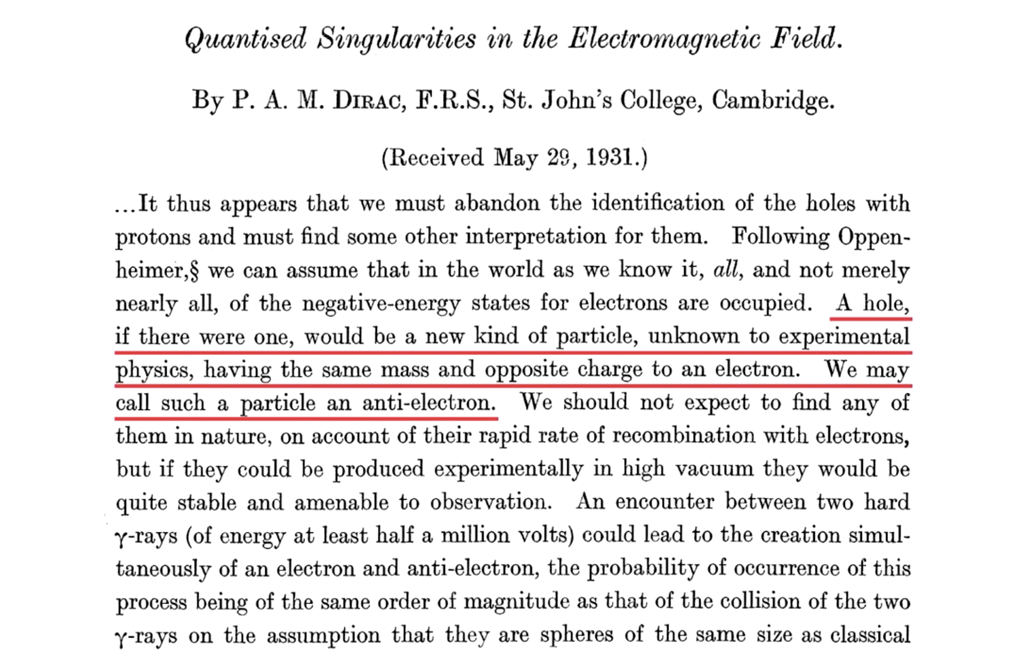
\includegraphics[scale=0.3]{img/diracPositrons.png}
\end{frame}

\begin{frame}
\frametitle{The discovery of the positron (Andersen, 1932)}

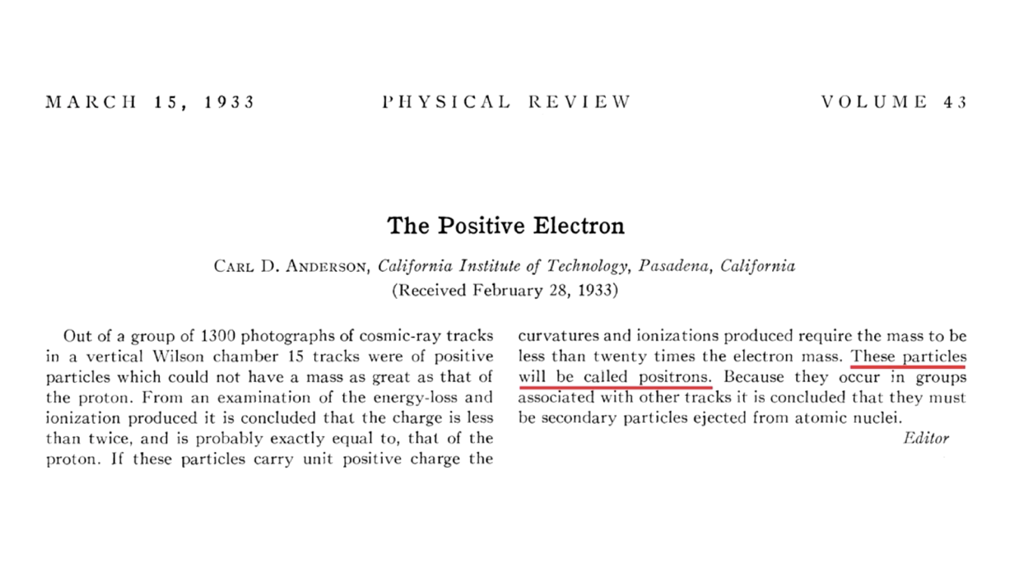
\includegraphics[scale=0.3]{img/AndersonPaper.png}
\end{frame}

%\begin{frame}
%\frametitle{The positron is real}
%
%\includegraphics[scale=0.3]{positronDiscovery.png}
%\end{frame}
%

%\begin{frame}
%\frametitle{The negative sea parable}
%
%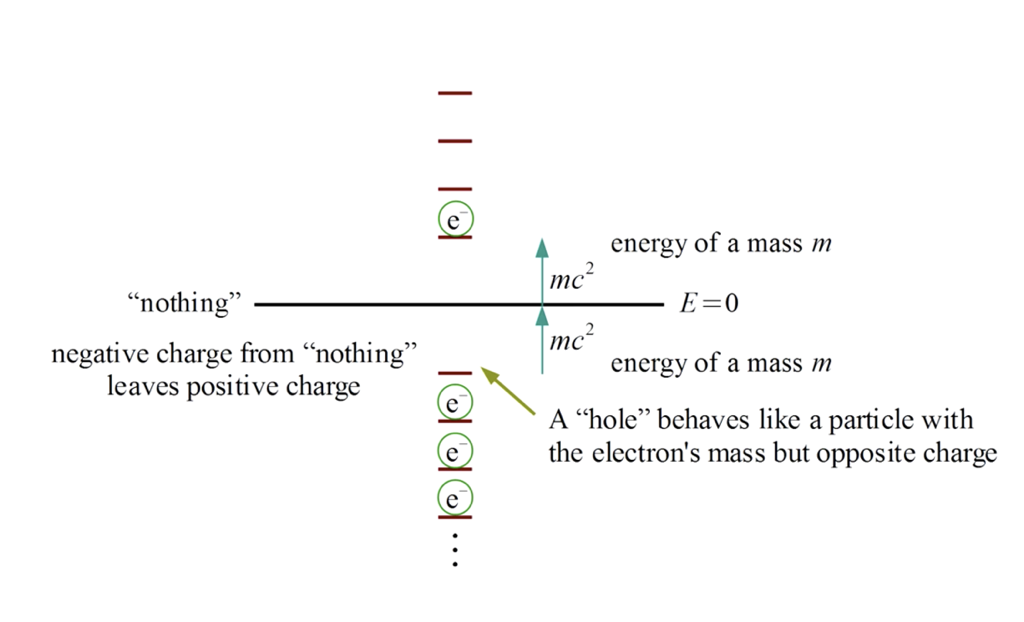
\includegraphics[scale=0.3]{img/negativeSea.png}
%\end{frame}

%\begin{frame}
%\frametitle{Relativistic quantum mechanics is not enough}
%
%\includegraphics[scale=0.3]{problemsRQM.png}
%\end{frame}
%
%\begin{frame}
%\frametitle{QFT for pedestrians}
%
%\includegraphics[scale=0.3]{FeymanDiagram.png}
%\end{frame}
%
%\begin{frame}
%\frametitle{QED diagrams}
%
%\includegraphics[scale=0.3]{QEDDiagrams.png}
%\end{frame}






